\section{Einleitung}

Beim Einbau von zweiwertigen Kationen in ein Gitter bestehend aus einwertigen Ionen entstehen elektrische Dipole. Diese können in Anteilen unter Einfluss eines elektrischen Feldes ausgerichtet werden. Ziel dieses Versuchs ist es den Relaxationsvorgang der ausgerichteten Dipole zu untersuchen und dabei die Aktivierungsenergie $W$ sowie die charakteristische Relaxationszeit $\tau_0$ des Materials zu bestimmen.

\section{Theorie}
\label{sec:Theorie}

Im Folgenden werden zunächst die theoretischen Grundlagen gelegt und dann das Messverfahren erläutert.

\subsection{Grundlagen}


\begin{figure}
  \centering
  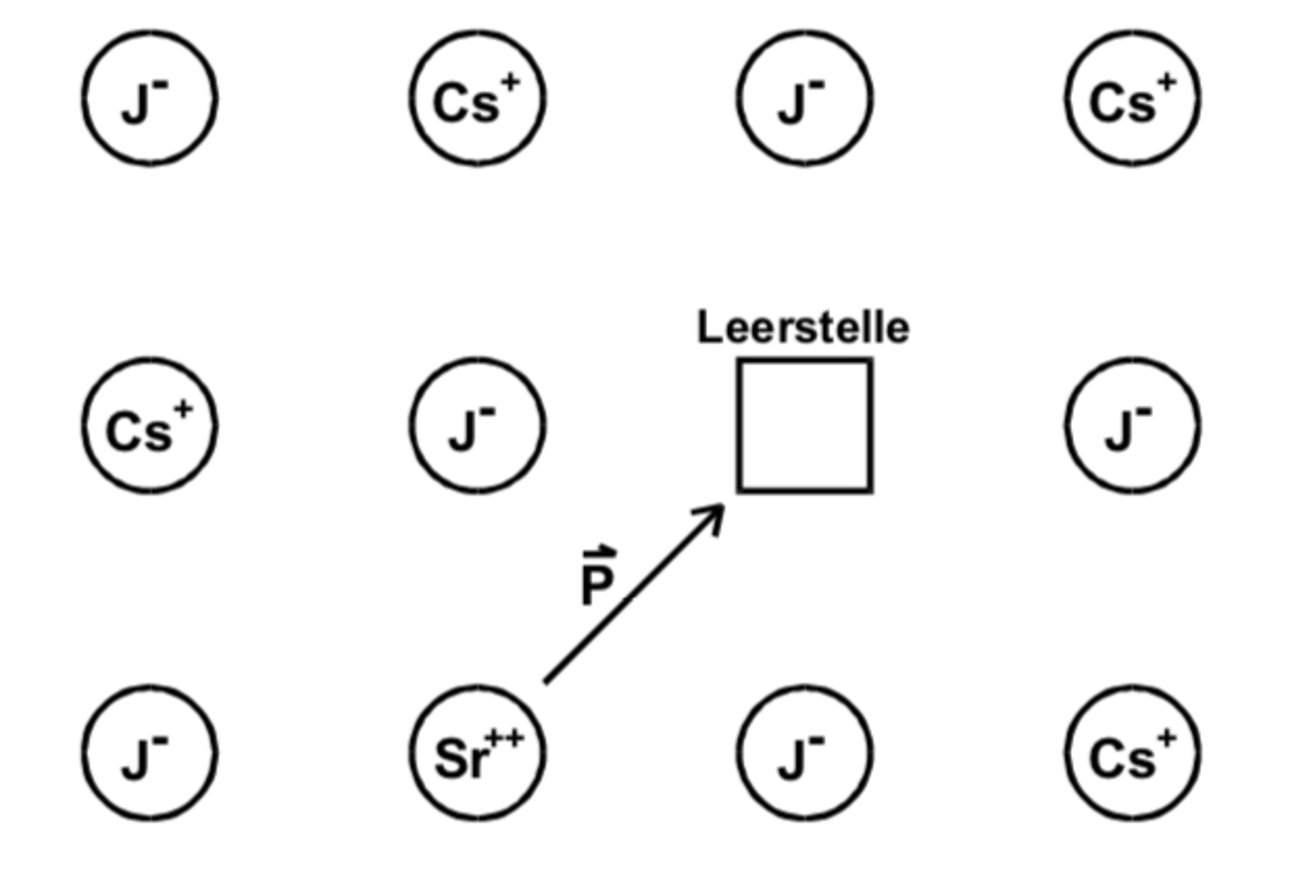
\includegraphics[height= 7cm]{BestNippelpiercings/gitter.pdf}
  \caption{Der elektrische Dipol in einem Ionenkristall nach Einbringung eines zweiwertigen Kations \cite{anleitung}.}
  \label{fig:gitter}
\end{figure}

In diesem Versuch wird Kaliumbromid untersucht, das mit Strontium dotiert ist. Durch die Dotierung entsteht aus Gründen der lokalen Ladungsneutralität eine Kationen-Leerstelle. Diese bildet mit dem Kation einen Dipol diskreter Ausrichtung wie in Abbildung \ref{fig:gitter} gezeigt. Es wurde gezeigt, dass unter \SI{500}{\celsius} nur Leerstellen in Kristallen wandern können \cite{wjost}. Damit eine Leerstelle wandern kann und sich somit die Ausrichtung des Dipols ändert, muss die Aktivierungsenergie $W$ aufgewendet werden. Die temperaturabhängige mittlere Zeit zwischen zwei Umorientierungen eines Dipols heißt Relaxationszeit. Sie folgt der Formel \eqref{eqn:relzeit}.
\begin{align}
  \tau(T) = \tau_0 \exp\left(\frac{W}{k_\text{B} T}\right) \label{eqn:relzeit}
\end{align}
Dabei gibt die Exponentialfunktion, der Boltzmannstatistik folgend, den Anteil der Dipole an, die aufgrund ihrer thermischen Bewegung die Energie $W$ besitzen und so ihre Richtung umkehren können.
Außerdem ist $k_\text{B}$ die Boltzmann-Konstante und $\tau_0$ die charakteristische Relaxationszeit, für die gilt: $\tau(\infty) := \tau_0$.

\subsection{Messverfahren}

Um zunächst die Dipole in der benutzten kreisförmigen Probe auszurichten, wird sie in das Feld eines Plattenkondensators eingebracht. Diese Ausrichtung wird allerdings durch thermische Bewegeungen gestört, sodass letzendlich nur der Bruchteil $y$ der Dipole ausgerichtet ist. Bei den gegebenen Versuchsbedingungen folgt dieser Anteil der Gleichung:
\begin{align}
  y(T) = \frac{pE}{3k_\text{B}T}.
\end{align}
Das Feld muss dafür allerdings über einen Zeitraum anliegen, der größer ist als die zu gegebener Temperatur geltende Relaxationszeit.
Der Anteil, der sich dann einstellt, kann durch schnelle Kühlung der Probe annähernd konstant gehalten werden, da dann die Relaxationszeit exponentiell zunimmt. Nachdem dann der Kondensator kurzgeschlossen wird, gleicht sich der bewegliche Ladungsanteil aus und die Ladung der Probe resultiert komplett aus den ausgerichteten Dipolen.

Wenn nun die Probe mit konstanter Heizrate $b$ erwärmt wird, sinkt die Relaxationszeit und die Dipole beginnen sich wieder statistisch verteilt auszurichten. Dies wird Dipolrelaxation genannt. Der bei der Umkehrung abfließende Depolarisationsstrom folgt dem Verlauf aus Abbildung \ref{fig:stromTemp}.
\begin{figure}
  \centering
  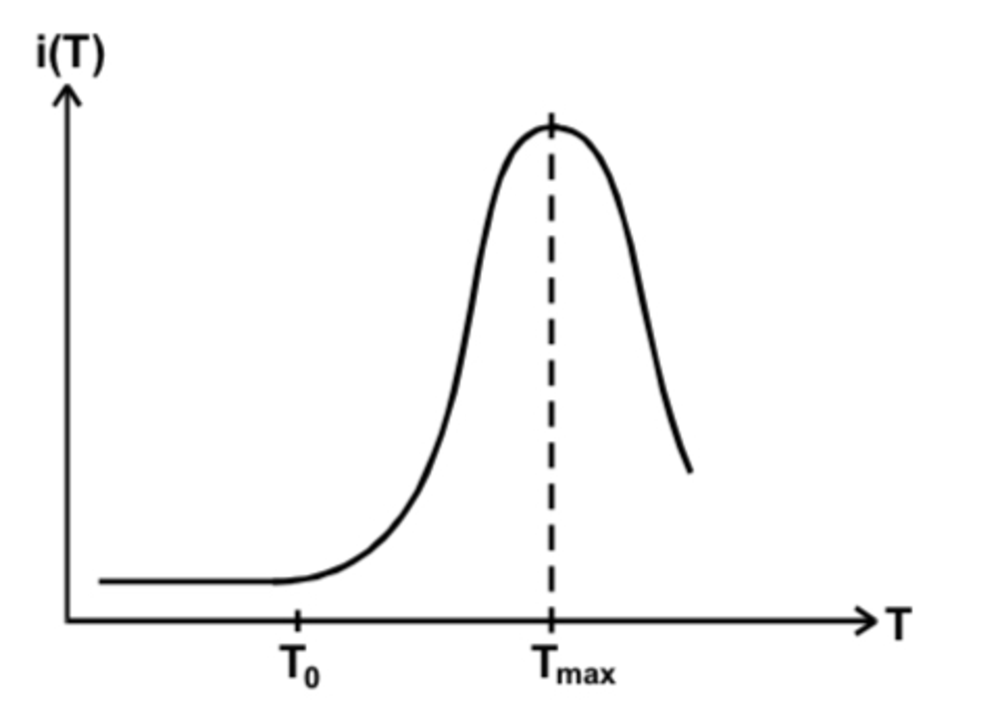
\includegraphics[height= 7cm]{BestNippelpiercings/stromTemp.pdf}
  \caption{Der Verlauf des temperaturabhängigen Depolarisationsstroms \cite{anleitung}.}
  \label{fig:stromTemp}
\end{figure}
Um aus den Strom-Temperatur-Messwertpaaren $W$ und auch $\tau_0$ zu bestimmen können zwei Wege unterschiedlicher Genauigkeit genutzt werden.
\begin{enumerate}
  \item Die allgemeine Formel für $j(T)$ lautet:
    \begin{align}
      j(T) = \frac{p^2 E N_\text{p}}{3k_\text{B} T_\text{p}\tau_0}
      \exp\left(-\frac{1}{b\tau_0} \int_{T_0}^T\exp\left(-\frac{W}{k_\text{B}T'}\right)\dif T'\right)
      \exp\left(-\frac{W}{k_\text{B}T}\right). \label{eqn:allgjt}
    \end{align}
    Hierbei ist $N_\text{p}$ die Anzahl an Dipolen zu Beginn des Aufheizens.
    Für den Anfangsteil der Kurve kann die Näherung
    \begin{align}
      j(T) \approx \frac{p^2 E N_\text{p}}{3k_\text{B} T_\text{p}\tau_0} \exp\left(-\frac{W}{k_\text{B}T}\right)
      \label{eqn:W1formel}
    \end{align}
    genutzt werden. In einem Diagramm, in dem $\ln(j)$ gegen $1/T$ aufgetragen ist, kann dann $W$ aus dem Anstieg bestimmt werden.
  \item Außerdem kann die Polarisation betrachtet werden und so die Gleichung
    \begin{align}
      \frac{W}{k_\text{B}T} = \ln\left(\frac{\int_{T}^{\infty} j(T')\dif T'}{j(T)\tau_0 b}\right)
      \label{eqn:W2formel}
    \end{align}
    hergeleitet werden. Durch Auftragen von
    \begin{align*}
      \ln\left(\frac{\int_T^{T^*} j(T')\dif T'}{j(T) \text{const}}\right)
    \end{align*}
    gegen $1/T$, kann $W$ aus dem Anstieg der ausgleichenden Geraden bestimmt werden. Dabei ist $T^*$ eine beliebige, feste Temperatur für die $i(T^*) \approx 0$ gilt, da dann der Relaxationsvorgang abgeschlossen ist.
\end{enumerate}
Die noch benötigte Größe $\tau_0$ kann durch Differentation der Gleichung \eqref{eqn:allgjt} erhalten werden. So kann $T_\text{max}$ der Relaxationszeit $\tau_\text{max}$ zugeordnet werden. Nach Einsetzen der beiden Werte in \eqref{eqn:relzeit} kann $\tau_0$ bestimmt werden.

% \subsection{Fehlerrechnung}
%
% Für die Fehlerfortpflanzung bei Gleichungen mit $N$ fehlerbehafteten Größen
% wird jeweils die Formel zur Gaußschen Fehlerfortpflanzung
%
% \begin{equation*}
%   \sigma = \sqrt{\sum_{i=1}^{N}\biggl(\frac{\partial f(x_{\g{i}})}{\partial x_{\g{i}}}
%   \sigma_{\g{i}}\biggr)^2}
% \end{equation*}
% mit der jeweiligen Funktion $f(x_{\g{i}})$, den Messgrößen $x_{\g{i}}$ und den
% zugehörigen Fehlern $\sigma_i$ verwendet.
% Zur Berechnung des arithmetischen Mittels von $N$ Messwerten wird jeweils die
% Formel
%
% \begin{equation*}
%   \bar{x} = \frac{1}{N}\sum_{i=1}^{N}x_{\g{i}}
% \end{equation*}
% mit den Messwerten $x_i$ benutzt.
% Die Standardabweichung des Mittelwerts wird jeweils mit der Gleichung
%
% \begin{equation*}
%   \bar{\sigma} = \sqrt{\frac{1}{N-1}\sum_{i=1}^{N}(x_{\g{i}} - \bar{x})^2}
% \end{equation*}
% mit den $N$ Messwerten $x_i$ berechnet.
%

% \cite{anleitung}
